%% *************************************************************************
%%
%% This is an RIT Space Exploration Standard defining guidelines for content
%% and formatting of project proposals.
%%
%% The document template SPEXformat.cls is based on the official IEEE LaTeX
%% class for authors of the Institute of Electrical and Electronics Engineers
%% (IEEE) Transactions journals and conferences.
%%
%% *************************************************************************

%% *************************************************************************
% LaTeX REFERENCES
% ----------------
%   Intro to LaTeX: http://www.rpi.edu/dept/arc/docs/latex/latex-intro.pdf
%   Comprehensive LaTeX symbol list: http://tug.ctan.org/info/symbols/comprehensive/symbols-a4.pdf
%% *************************************************************************

% tell \LaTeX what kind of formatting to use
\documentclass[journal]{SPEXformat}
% enable math package for equations
\usepackage{amsmath}
% enable placeholder text generator
\usepackage{blindtext}
% enable toolbox for embedding figures and pictures
\usepackage{graphicx}
% enable package for adding a list of variables and constants at the beginning, aka "nomenclature"
\usepackage{nomencl}
% enable package for easily formatting units
\usepackage{siunitx}
% enable package for cross-referencing figures, sections, references etc.
% how to use hyperref: http://www2.washjeff.edu/users/rhigginbottom/latex/resources/lecture09.pdf
\usepackage{hyperref}
% change text encoding to make it more crisp
\usepackage[T1]{fontenc}
% enable conditionals for help text
\usepackage{etoolbox}

% ----------------------------
\newbool{showhelp}
% ~~~~~~~~~~~~~~~~~~~~~~~~~~
% SHOW HELP TEXT IN THE PDF?
\setbool{showhelp}{false}
% ~~~~~~~~~~~~~~~~~~~~~~~~~~
% define conditional help text environment
\newsavebox{\helpbox}
\newenvironment{help}{
  \ttfamily\footnotesize\sloppy
  \begin{lrbox}{\helpbox}\begin{minipage}{\linewidth}
  }{
  \end{minipage}\end{lrbox}
  \ifbool{showhelp}{
    \fbox{\usebox{\helpbox}}
  }{}
}
% ----------------------------

% initialize nomenclature package
\makenomenclature{}

% set title. choose something as descriptive and precise as possible. Descriptive > sounding cool. remember this!
\title{Characterization of Habian Motion}
\author{
  \begin{help}
    List the authors of the proposal. The Champion should go first.
    The \$~\$ markers tell \LaTeX{} to treat the text inside to be treated as a math expression. This way you can use operators like \textcaret{} to place characters as superscripts.
    The \textbackslash{}thanks command puts the contents inside those brackets in a footnote at the bottom of the first page. Technically speaking, \textbackslash{}thanks is just a specially formatted footnote.
    Read here for a more advanced options:  \url{http://tex.stackexchange.com/questions/826/symbols-instead-of-numbers-as-footnote-markers}
  \end{help}
  James~Emerson~Parkus$^{*\dagger}$%
    \thanks{$^{*}$Project Champion}%
    \thanks{$^{\dagger}$BS '20, Mechanical Engineering Technology \& BS '22 Physics}

  % the recommended order for symbolic footnotes is
  %   (1) asterisk        *   *
  %   (2) dagger          †   \dagger
  %   (3) double dagger   ‡   \ddagger
  %   (4) section symbol  §   \S
  %   (5) paragraph       ¶   \P
  %   et cetera. For higher counts, use 2x symbols (1)-(5) (i.e. (6) two asterisks **). Keep cycling through (1)-(5) using 3x, 4x, and so on.
  %   Note that these symbol codes work in math mode and text mode.
  %   There are ways to make LaTeX do this for you, but it is more advanced and not entirely necessary, especially for short author lists. Not worth the hassle, in my opinion.
}
% page header for pages other than cover page
\markboth{Project Proposal Standard}%
{Linden \MakeLowercase{\textit{et al.}}: RIT Space Exploration}

% Initial setup is over, start building the document itself
\begin{document}
\maketitle%
% correct bad hyphenation here, separated by spaces
\hyphenation{explor-ation}

\begin{abstract}
  This project would be for the RIT SPEX High Altitude Balloon team. The goal is to create a map of the HAB condtions throughout
  flight. This would be extremely benefical when creating a HAB for an experiment. Being able to understand "habian" motion
  can allow the project engineers to adequately design the payload to survive flight conditions.
    \begin{help}
      The abstract is a brief summary of the proposal. Typically it includes the purpose of the proposal, key goals or objectives, and justifications.
      Be sure not to confuse the abstract with the introduction.
      It is easiest to write the abstract after the rest of the paper has been written.
      That way you can choose key information from the sections that you've already completed and string them together in the abstract.
      Consider the abstract to be your elevator pitch to anyone reading this proposal.
      What are they reading?
      What is the goal?
      Why is it worth my time?
      The abstract is what will show up in Google results and other search engines, and what people will read when they are deciding what is worth their time and brain power.
    \end{help}
\end{abstract}

\label{sec:nomenclature}
\newcommand{\nomunit}[1]{%
\renewcommand{\nomentryend}{\hspace*{\fill}#1}}
\renewcommand{\nompreamble}{
  \begin{help}
    If you include mathematical expressions or express variables in the proposal, list them with their corresponding definitions here as a list.
    The two lines below make it look nice when defining units/values to constants.

    Note that math terms and non-math terms are separated and alphabetized, regardless of the order in which they are defined. (Recall terms \$like this\$ are in the math environment)
    Read more about advanced nomenclature formatting here:\\
    \url{https://www.sharelatex.com/learn/Nomenclatures}
  \end{help}
  }
\nomenclature{RIT}{Rochester Institute of Technology}
\nomenclature{SPEX}{RIT Space Exploration}
\nomenclature{SPP}{SPEX Project Proposal}
\nomenclature{HAB}{High Altitude Balloon}

\printnomenclature{}
\begin{help}
  The sections included here are required. Additional sections and subsections may be added as necessary.
\end{help}
\section{Introduction}
\label{sec:introduction}
\begin{help}
  The introduction is a place to give background and context before diving into the subject matter.
  Establish context for the work you are about to propose and the main ideas of the proposition itself.
\end{help}

\IEEEPARstart{H}{igh} altitude balloons are scientific experiments that allow teams to test experiments in \textit{space-like} conditions.
  Of course, this is only one type of many types of possible high altitude experiments. During the course of experiment
  design the team must include flight conditions in there engineering requirements. High altitude balloons are swung,
  twisted, and rocked during flight. What are the accelerations? What are the G's that the payload experiences?
  That is question this project will answer. This project will enlighten our understanding of how a high altitude balloon
  is affected during flight by the conditions of the atmosphere at any given location throughout. Hence, the idea
  of creating a map of habian motion.

\section{Primary Objective}
\label{sec:primary-obj}
\begin{help}
  At the end of the day, whether the project ``succeeds'' or ``fails'' is judged against the objectives it sought to meet.
  Note that results that contradict expectations/hypotheses are not failures if the scientific \& engineering methods are followed along the way.
  Sometimes our expectations are wrong and that can be just as successful as getting data we thought we'd see.
  What matters are what questions you intend to answer.
  This is the main purpose or main goal the project hopes to achieve.
\end{help}
  The \textit{characterization of habian motion} project goal is to create a very detailed document, along with a
  visual component, that will allow all HAB teams around the world to understand the types of conditions that
  there HAB will endure through flight. The document will include many different components of HAB conditions (this will be
  further explained in the following secions). A few of these components are rotation and the acceleration in
  three dimensions. These can define the forces on the HAB during flights which in turn defines the necessary fixturing
  that the internal components of the HAB must have.


% \section{Secondary Objectives}
% \label{sec:secondary-obj}

\begin{help}
  Secondary Objectives are lower priority or bonus objectives that are significant but not the main focus of the project. This template does not have secondary objectives.
\end{help}

\section{Project Description}
\label{sec:benefit}
\begin{help}
  [this help section is not yet defined]
\end{help}
  This project will rely on sensor data. As this will be our main form of data collection. For this project will want to
  collect as many forms of data as we can. This data includes the following; Rotational Acceleration, Acceleration in the
  x y z axis, temperature, thermal diffusivity, ambient pressure, wind velocity, \textit{pendulum-like} motion, and altitude.
  Now, the RIT SPEX team has collected some of this data before but it is not adequate. The sensors are shielded within the HAB.
  This is good for component survival however it has dampened that data collection, such as temperature, pressure, etc.
  This time, the sensors will be exposed to the atmosphere, at least the ones that must be. The mechanical data collection
  does not need to be exposed to the atmosphere, including the dimensional accelerations and pendulum motion.
\begin{help}
  Below I have used subsections to identify key ideas in this section. These particular subsections are not required as part of the SPEX Standard, but serve as an example of using subsections in a text.
\end{help}

\subsection{Atmospheric Data}
\label{subsec:atmospheric data}
  The data that must be collected from the atmosphere are; temperature, atmospheric pressure (aka ambient pressure),
  thermal diffusivity, wind velocity, and solar intensity. The temperature is very important because all materials have
  an operational temperature. Once these temperature boundaries are breached the material's itegrity is
  compromised. Another very important condition is the ambient pressure. This pressure is important for understanding
  how electrical operations should be designed as the altitude increases. As altitude increases the diffusivity of
  thermal radiation made by the electronics changes and can create problems for the components such as overheating.
  Wind velocity is a mechanical component of flight, but, needs to be measured on the outside of the balloon independently
  of the other mechanical data collections. Lastly, the solar itensity must be measured. This is not temperature.
  The solar intesity is the thermal energy transmitted to the HAB from photons. As the ambient pressure decreases
  the energy of incoming photons increases, maybe not a lot but any measureable difference is important because future
  HAB electrical components may be very sensitive to this type of radiation.

\subsection{Mechanical Data}
\label{subsec:mechanical data}
  The mechanical data that must be collected are; accelerations in the x y z dimensions independently, rotational acceleration
  , and pendulum acceleration. The accelerations in the x y z dimensions are of critical importance. This is the most
  definitive accelerations that we can use in the map of habian motion. The acceleration of the HAB in these dimensions
  will allow the HAB teams to understand the force to which the HAB is subjected. The acceleration in the angular sense
  is also of critical importance as this can cause many mechanical failures in the sense of securement. The twisting of
  wires or thread can cause torsional stress which after a certain amount of rotations can enter a non-newtonian situation
  that can cause incredible stress. This unanticipated stress can be the root of mechanical failure. Lastly, the data
  collection of the pendulum motion. HABs are mostly commony secured to the balloon through thread. When wind is applied
  to the HAB the resulting motion is analogous to a pendulum. This can be the root of a new type of stress. And as we know,
  stress is additive so it is important to understand all possible stresses that to which the HAB could be subjected. The
  pendulum equation can be easily utilized to analyze the stresses. But to do this we need to know two indpendent variables,
  theta (the angle through which the HAB moves) and the acceleration. Then we can apply the mathematical equation \ref{pendulum}.

  \begin{equation} \label{pendulum}
  \frac{d^2\theta}{dt^2} = -\frac{g}{l}\sin(\theta)
  \end{equation}

  % use \ref{pendulum} to put the equation in the text
\section{Mechanical Design}
\label{sec:mechanical design}
\begin{help}
  What path do you anticipate the project to take?
\end{help}

\subsection{Description}
\label{subsec: description}
  The mechanical design will feature a foam box. The dimensions of which will depend mostly on the necessary size of
  pcbs and the necessary length of the pendulum as well as the height of the deck plate camera. The pcbs will need to
  have accelerometers to measure acceleration in the x y z directions and around its center of mass (rotation). There
  is no accelerometer to measure the pendulum effect. So we employ a possible solution. This possible solution includes
  putting a pendulum in the HAB with a comparitively massive object on the end (compared to the mass of the pendulum
  mass per unit length). When the HAB swings the pendulum in the HAB will always point towards the center of the earth.
  So, we can figure out the swept angle using the equation~\ref{sweep angle}.

  \begin{equation} \label{sweep angle}
  \theta = \arccos(\frac{m}{l})
  \end{equation}

  Where m is the x-component of the pendulum length vector. This will allow us to use equation~\ref{pendulum} to find
  the acceleration of the HAB and we can measure its mass so we can find the force of tension in the lacing chord
  connecting the HAB to the balloon (this assumes the parachute is the same as the lacing chord).

\subsection{Design}
\label{subsec: design}

  The HAB will be secured in a net of nylon straps. This will ensure stability and mechanical safety as the nylon
  temperature range is approximately negative 40 degrees to positive 390 degrees fahrenheit. Although the temperatures of the atmosphere that the HAB
  travels through drop below negative 50 degrees, this should not be a problem as long as the weight that the nylon
  net holds is within its tensile limits and the HAB does not remain in that part of the atmosphere for a long
  duration.
\begin{figure}
  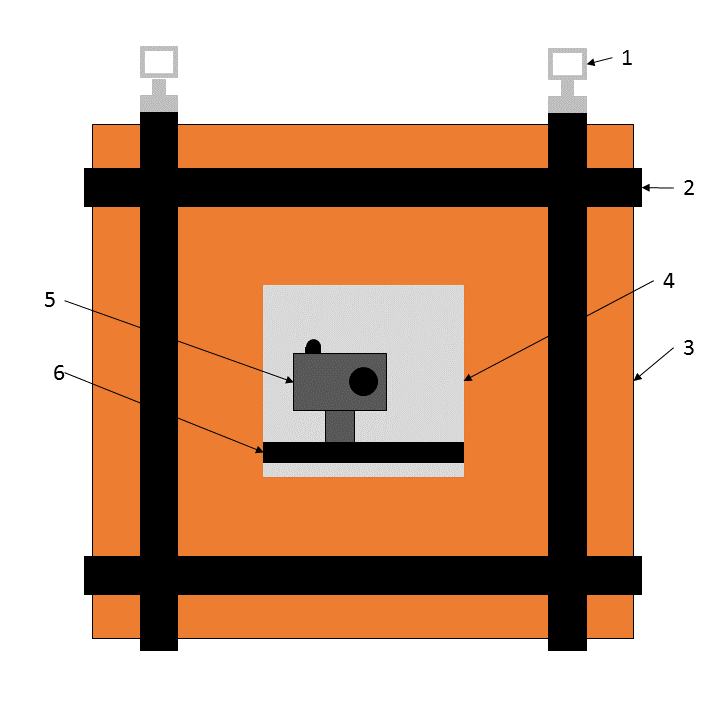
\includegraphics[width = \linewidth]{figs/HAB-Strap-Fig.png}
  \caption{A front view of the high altitude balloon payload.}
  \label{fig:HAB Front View}
\end{figure}

  In figure 1 the HAB Structural Design is displayed. There are parachute connections [1], nylon straps
  [2], the payload [3], a plexi-glass window [4], a GoPro [5], and a deck plate [6]. There is also a new connection
  proposal for the nylon net. It will be for connecting the nylon straps together for a quick-release mechanism.
\subsubsection{The Parachute Connections}
\label{subsubsec: the parachute connections}

  The parachute connections are made out of aluminum for strength and reduncey. The main reason for the aluminum is because these connections
  must have a high factor of safety. If the parachute connections fail, the HAB plummets to the ground at an increasing
  velocity [until terminal velocity is achieved] and will certainly be destroyed while posing a safety threat to
  pedestrains. The connections are an assembly of two pieces secured by a 1/4-20 socket cap screws that is counterbored
  into the bottom piece so it does not protrude from the part and harm the surface of the HAB. Loctite will also be applied
  to ensure the screws do not rattle loose.
\subsubsection{The Nylon Straps}
\label{subsubsec: the nylon straps}

  The nylon straps are to be woven into a cross-netting arrangement for pressure distribution across the surface of the HAB
  payload. Nylon was chosen because of its heritage with HAB payload securement. The nylon will be stitched at a few
  intersections that coordinate properly with the corners as displayed in figure 1. The nylon strap will alleviate the
  personal stress entailed in the setup and launch of the RIT SPEX HAB Icarus mission payload. The nylon straps will have
  an aluminum connection that can be easily removed and vis versa. It is important that the nylon straps are appropriately
  tight around the payload as to not severly damage the outside of the HAB payload, while maintaining the structural
  integrity.
\subsubsection{The Plexi-Glass Window/Gopro Integration}
\label{subsubsec: the plexi-glass window/gopro integration}

  For this mission understanding the conditions of flight is the primary goal. Sometimes the human eye can allow teams
  to judge certain conditional circumstances that a sensor simply cannot, such as rain effect on the HAB [surface-wise].
  To observe the conditions in such a manner a GoPro will be employed to record the entire flight. On past RIT SPEX HAB
  payloads and launches complications with the GoPro were a constant bother. It shutoff on the Icarus mission shortly
  before descent. The running theory for this failure is that the GoPro became too cold and the camera shutoff as a
  homostasis policy. To help alleviate this possiblity the GoPro will be wrapped in thermal wrap which will help the GoPro
  insulate itself through flight and it will be inside the HAB payload. The GoPro will be able to record the outside
  of the HAB through a plexi-glass window that will be adhesively bonded to the HAB payload. The design can be seen in
  figure 2.

\begin{figure}
  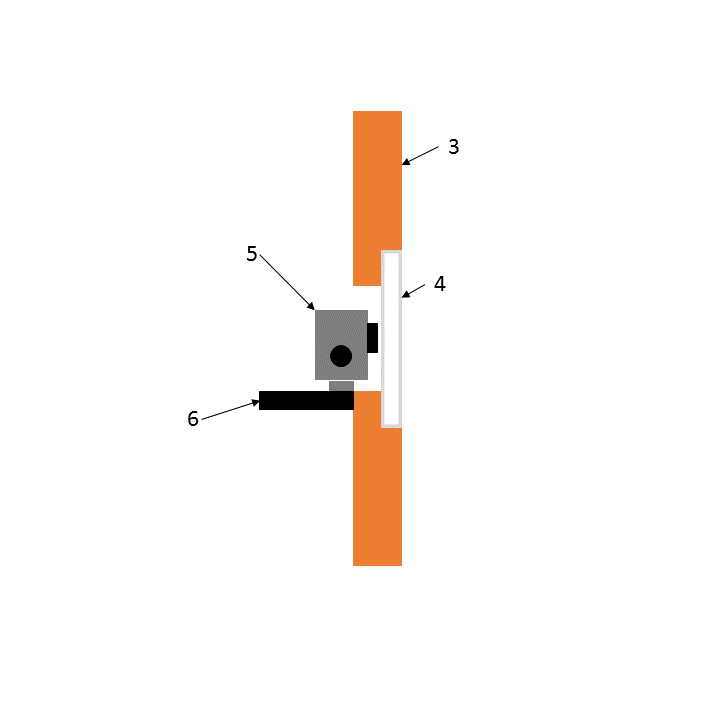
\includegraphics[width = \linewidth]{figs/GoPro-Fig.png}
  \caption{A section view of the gopro secured in the HAB.}
  \label{fig: GoPro Section View}
\end{figure}

  The GoPro will likely see the edge of the HAB payload because the angle of viewing is very large. Although, this should
  be fixable with simple video editting. Inside the HAB payload the GoPro will be fastened to a deck plate likely made out
  of 3D printed PLA or ABS. An aluminum plate may be necessary to keep the GoPro stable during the intense vibrations
  and forces sustained throughout flight. The GoPro is \textit{top heavy} so it may repeat a performance from RIT SPEX HAB
  mission Icarus where it is knocked to a signifcantly different viewing angle to the point where the video footage is
  partial and mostly useless.
\subsubsection{The Payload Deck Plate}
\label{subsubsec: the payload deck plate}

  The GoPro will sit on a deck plate inside the HAB payload. 3D Printing a rack such as the one designed by David Breen
  for the fourth RIT SPEX HAB mission. The rack can be simplifed because all that will be needed is two levels, one for the
  GoPro and one for the pendulum-camera system. There should be plenty of space for the necessary pcbs, as the HAB payload
  base geometry is a cube, which pcbs can conform to very easily. The second level will be mostly clear except for the
  GoPro, allowing more space for the pcbs to sit.
\subsubsection{The Nylon Strap Connector}
\label{subsubsec: the nylon strap connector}

  The nylon strap connector will allow the nylon straps to connect from either ends to be easily fitted around the HAB
  payload. They will be made out of aluminum as they are as integral to the structural integrity of the HAB payload
  as the parachute connectors are. They keep the nylon net around the HAB payload throughout flight. It is convinent
  to make them out of aluminum as they have a relatively simplistic geometry that can be easily manufactured on a
  milling machine. See figure 3 for a reference to its geometry.

\begin{figure}
  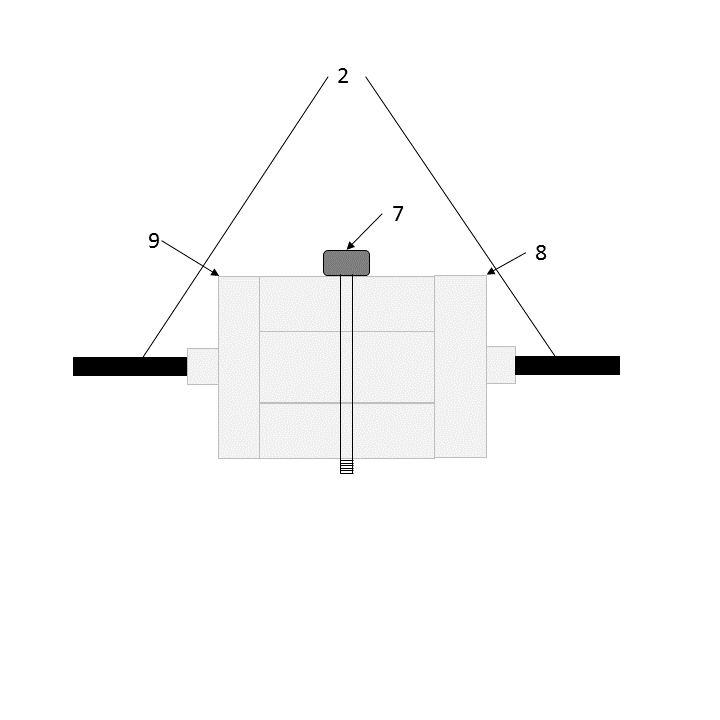
\includegraphics[width = \linewidth]{figs/Nylon-Aluminum-Fixture-Side-Fig.png}
  \caption{A side view of the aluminum nylon strap connector.}
  \label{fig: Nylon Strap Connector}
\end{figure}

\begin{figure}
  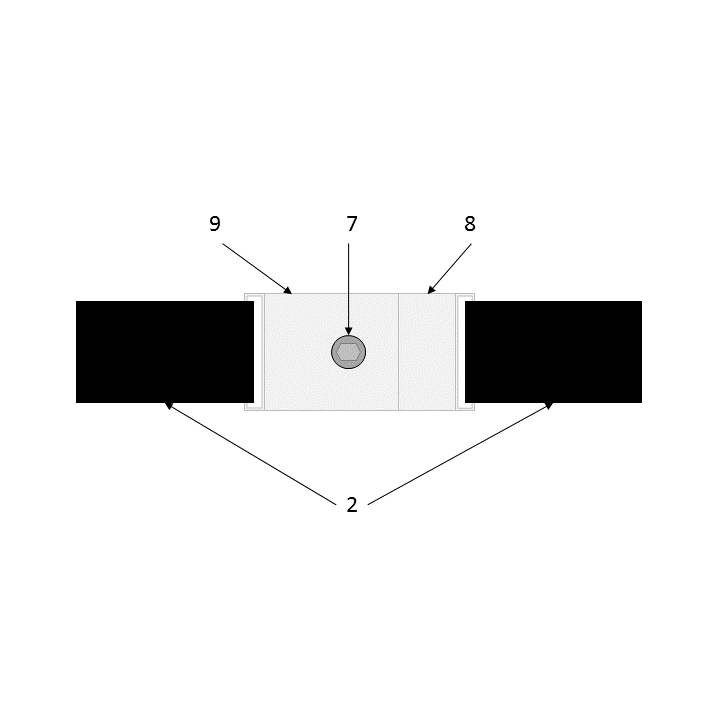
\includegraphics[width = \linewidth]{figs/Nylon-Aluminum-Top-Fig.png}
  \caption{A top view of the nylon strap mechanism.}
\label{fig: Nylon Strap Top View}
\end{figure}

  There are two parts. One with a \textit{U-like} geometry [9] and one with a \textit{pin-like} geometry [8]. They fit together
  like a simple plastic clip, except more rectangular and made out of aluminum. Each is attached to one end of the nylon
  strap and the nylon strap is put through the rectangular hole on each part. Then the nylon strap is stitched with high-tensile
  strength thread when folded through the hole. There will be a 1/4-20 socket cap screw [7] that threads through the two pieces and can be secured with a nut or can
  just be threaded into aluminum. The latter is recommended as a nut may damage the side of the HAB payload. Flat and
  lock washers will be added to the 1/4-20 screw for reduncey. See figure 4 for a top view of the strap mechanism.

\section{Avionics \& Data Collection}
\label{sec: avionics and data collection}

  An important part of any high altitude balloon launch is tracking the balloon. This allows the team to attempt payload
  recovery or signal for local HAM operators for help in honing down the exact landing location. Using APRS or a GPS
  system usually entails signal loss under 1000 - 10000 feet, because mountains usually cut off the signal.
\subsection{Geolocational Tracking and Recovery }
\label{subsec: geolocational tracking and recovery}

  For this HAB launch, recovery is essential. It is unlikely we will be able to transmit the all the data to the ground
  station. This is mostly because of the signal loss expected below 1000 feet, since impact conditions are critical
  for the mission statement. For redundency we will have a geolocational positioning system [GPS] and an automatic packet
  reporting system [APRS]. Local HAM operators will be asked to help in the exact positioning of the HAB payload.
  Once the location is known a designated team of HAB-Hunters will retrieve the payload. Immediately prior to launch,
  the team will return to mission control to track the HAB's trajectory. One monitor will be designated to following
  the APRS data and another will be designated to viewing the trajectory in three dimensions on Google Earth$^\textregistered$.
  This three dimensional trajectory can be saved and cataloged while being used for a better visualization when discussing
  the HAB mission.
\subsection{Avionics \& Data Collection}
\label{subsec: avionics and data collection}

  The avionics for this payload will include creating and populating mutliple pcbs for decreased design complexity to
  allow high degree of confidence in the functionality of the boards. The pcbs must include a IMU for gravitational
  tracking. This allows a fixed radial vector that can be used for more advanced data analysis. There will be a sensor for
  temperature and ambient pressure. It must also include rotational acceleration sensor and a three dimensional acceleration sensor [x y z]. There will
  also be a fully functioning solar panel. It will be placed on the side [except the GoPro side] and the rate at which
  it absorbs the kinetic energy of the solar photons will be recorded and analyzed.
  Concerning the available space for pcb placement, there will be very few other objects inside the payload. There will certainly
  be a GoPro for video footage, a pendulum for tracking the sweep angle, and a smaller camera designated to recording the
  moion of the pendulum. The pcbs will likely have the entirety of the bottom deck plate [which will have an abs cover for
  to allow the pcbs to connect through standoffs. The second deck plate will also be made of abs for similar reasons.
\subsubsection{Pendulum Motion Data Collection}
\label{subsubsec: pendulum motion data collection}

  A difficult part of this mission will be correcting calculating the pendulum forces on the HAB payload. This is important
  for finding the extra strain placed upon the parachute-payload connection. This includes the aluminum connections and the
  thread. It will also allow further analysis into the wind conditions. Because the x y z sensors will only capture the
  wind-caused accelerations for a couple seconds. This is because when the payload starts to move, the radial connection to the balloon will cause
  the payload to swing as a pendulum. This can skew the data if constant cross-product [between radial vector (moment arm) and wind force]
  are assumed. The torque of the HAB payload is determined by $\vec{r}$ x $\vec{F}$.

  The solution to finding the sweep angle of the payload [angular displacement from vertical axis] will be tracking
  the motion of the HAB payload pendulum with a video. The pendulum will hang a heavy mass and when the HAB payload swings
  to the side, the pendulum inside the HAB payload will seem to swing [even though it is a constant angle with respect
  to an outside observer]. Once the pendulum reaches its maximum amplitude it will be measured using a caliper or a ruler.
  There will be a series of circles drawn on the inside of the lid of the payload. They will have varying radii and using these
  radii the projection of the length vector onto the local x-axis [parallel to HAB lid] will yield the necessary data
  to calculate the swept angle. See figure 5 for a representation of these vectors. The projected vector is created
  by projecting $\vec{l}$ onto $\vec{t}$. The $\vec{h}$ serves a representation of the local vertical [y axis].

\begin{figure}
  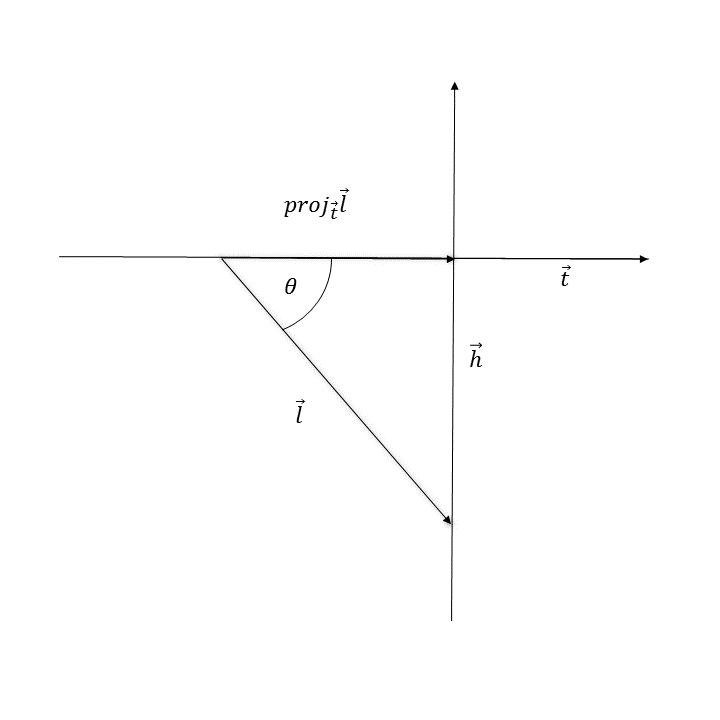
\includegraphics[width = \linewidth]{figs/HAB-Pendulum-Projection.png}
  \caption{A representation of the projected vectors and the sweep angle.}
\label{fig: HAB Payload Pendulum Projection}
\end{figure}

\section{Summary \& Conculsion}
\label{sec:summary and conclusion}

  The ultimate goal of this mission is to create a very detailed and extensive report on HAB flight conditions
  as a function of several arguements [a HAB flight map]. For the best results, testing in different weather conditions and overall environments
  will yield more data that can cover a wider range of HAB experiments. For the first flight a single arguement for the HAB map
  will suffice, the arguement being altitude. As other experiments are conducted, other arguements will be available,
  such as average humidity, heat, or average regional temperature.

  After this map is created, HAB teams all over the world
  can use it for creating a HAB structural design. It will be a great opportunity for SPEX to have their name on such a document.
  And it is a very plausible mission with a high level of feasibility as much of the necessary instrumentation has been flown
  and used on the previous SPEX HAB missions.
\section*{Acknowledgements}
The author would like to thank Dr.~Bill Destler for being an exemplary human.

\onecolumn
\appendices{}


\end{document}
